%! Author = tstreule

\section{Computed Tomography}

Quantitative with \textbf{Houndsfield unit} (normed to water):\\
\highlight{$\displaystyle \textrm{CT value} = \frac{\mu - \mu\ped{water}}{\mu\ped{water}}\cdot \unit[1000]{HU}$}

Beam types: Pencil, Fan, Parallel fan, cone.

\textbf{Algebraic Reconstruction}:
Out of a $n \times n$-Image, make a $n^2 \times n^2$ equation system:
$\vec{P} = W \vec{\mu}$ (P are the measurements, W are the weightings, how much a beam crossed a box/pixel)\\
\highlight{$\displaystyle \vec{\mu} = (W^H W)^{-1} W^H \vec{P}$} $~^H$: hermetisch transponiert.

\textbf{Projection Slice Theorem}: Project a 2D function onto a line and do a 1D Fourier transform \quad $\iff$\\
Do a 2D Fourier transform of that 2D function and slice it through its origin (parallel to the line above).
%%%%%%%%%%%%%%%%%%%%%%%%%%%%%%%%%%%%%%%%%%%%%%%%%%%%%%
\subsection{Backprojection}
%
When doing simple Backprojection: $PSF = \frac{1}{|r|}$

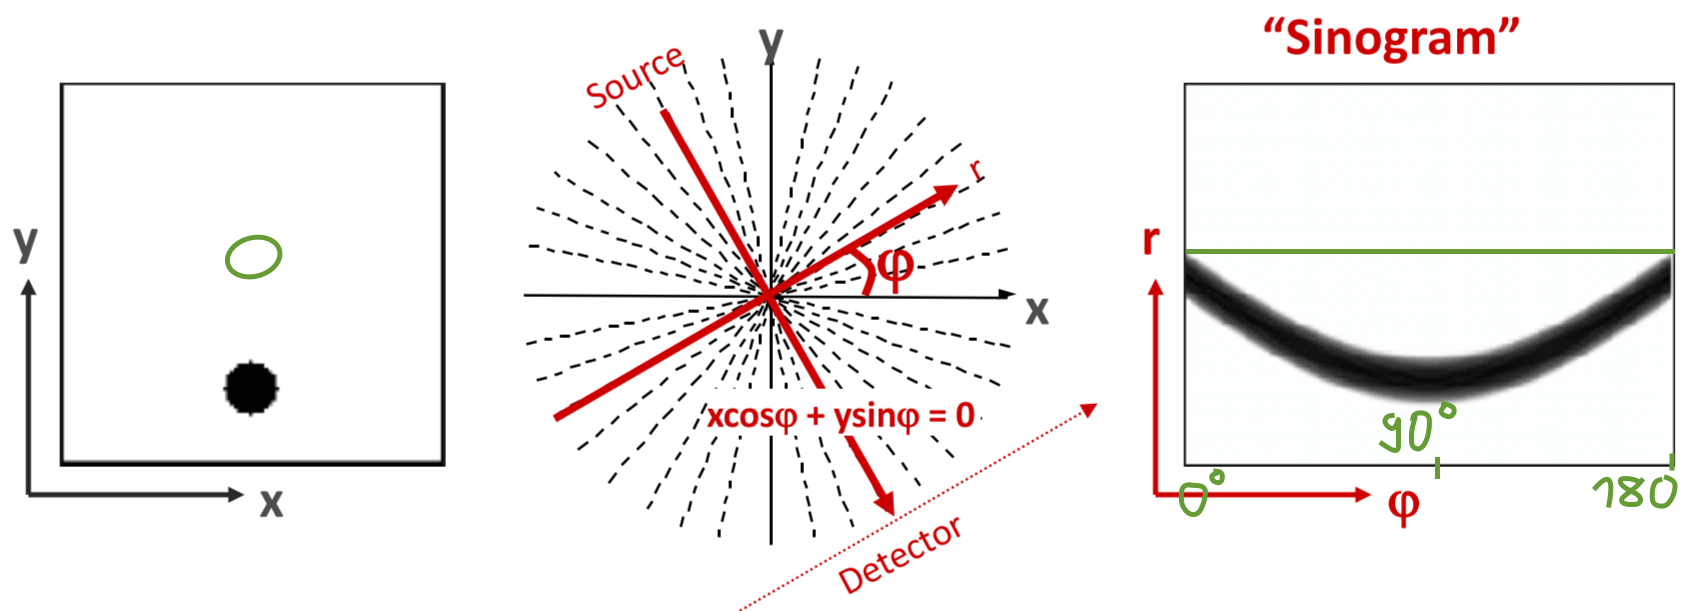
\includegraphics[width = .8\linewidth]{CT_Sinogram}\\
$P_\phi(r) = -R[\mu](r, \phi) = -\iint \limits_{-\infty}^\infty \mu(x, y) \delta(\underbrace{x \cos \phi + y \sin \phi - r\vspace{-1mm}}_{\text{line formula}\vspace{-1mm}})dxdy$

Math. Deduction: \textbf{1st Reconstruction formula}:\\
Projection $P_\phi(r) = -\int \mu(r, s) ds$\\
$\mathcal{F}\{P_\phi(r)\}(u,\phi) = \int P_\phi(r) e^{-jur}dr =$\\
$= - \iint \mu(r, s) e^{-jur} dr ds =$ (with $r = x\cos \phi + y \sin \phi$)\\
$= -\iint \mu(x, y) \exp(-jx\underbrace{u \cos \phi\vspace{-1mm}}_{\vspace{-2mm}p \hat{=} k_x} - jy\underbrace{u\sin\phi\vspace{-1mm}}_{\vspace{-2mm}q \hat{=} k_y}) dxdy = $\\
$= - \iint \mu(x, y) e^{-jxp - jyq} dx dy$ (until here just proj. slice th.)\\
\highlight{$\displaystyle \implies \mu(x, y) = \frac{-1}{4\pi^2}\iint \mathcal{F}\{P_\phi(r)\}(p, q) \eu^{\iu xp + \iu yq} \diff p\diff q$}\\
Fill k-space with $\mathcal{F}$ of the proj.s $\hat{=}$ Backproj. of $\mathcal{F}$\\
Then do 2D-backtransformation

\textbf{2nd variant}: Change of integration variables:\\
\fbox{$u(x,y) = \frac{-1}{4\pi^2} \int \limits_0^\pi \int \limits_{-\infty}^\infty \mathcal{F}\{P_\phi(u)\}\eu^{\iu ur} \abs{u} \diff u \diff\phi$}

\textbf{Filtered Backprojection}:\\
$\highlight{\hat{u}(x, y) = \int_0^\pi P_\phi \cdot \mathcal{F}^{-1} \{|u|\} d\phi} = \sum_{j=0}^n \big( p(r,\varphi_j)*h(r) \big) \textrm{d}\varphi$.
%%%%%%%%%%%%%%%%%%%%%%%%%%%%%%%%%%%%%%%%%%%%%%%%%%%%%%
\subsection{Effects that occur in practice \& Spiral CT}
``Streak artifacts'': Too few projections have been acquired. Correction: Additional low-pass $\implies$ SNR rises.

``data grabbing'': Convert cartesian $\leftrightarrow$ polar coordinaates

Filter in image-domain: $|u| \quad \laplace \quad \frac{1}{(2\pi r)^2}$\\
If Fourier-domain is band-limited, the filter becomes a \textbf{Ram-Lak}: $\mathrm{sinc}(r) * \frac{1}{(2\pi r)^2}$
\quad\textcolor{gray}{(don't forget: $\mathrm{rect}(r) \quad\laplace\quad \mathrm{sinc}(r)$)}

Have other filter, in order to not amplify noise: \textbf{Shepp-Logan, Cosine or Hann-Filter}, i.e. combine with low-pass.

\textbf{Spiral CT}: Before backprojection, do linear interpolation of data. \textbf{Pitch}=1: The neighboring slices touch, Pitch=2: slice distance = 1 slice thickness
%%%%%%%%%%%%%%%%%%%%%%%%%%%%%%%%%%%%%%%%%%%%%%%%%%%%%%
\subsection{(Quantum) Noise}
%
Distribution of photon counts is $P_\lambda(x)$.
$\textrm{E}\{P_\lambda\} = \lambda \equiv \bar{N}$, $\sigma = \sqrt{\lambda}$.\\
$\!\implies \textrm{SNR} = \frac{\textrm{average}}{\textrm{std. deviation}} \!=\! \frac{\overline{N}}{\sqrt{\overline{N}}} = \sqrt{N}$\\
\phantom{$\!\implies$} where $N$: \#X-rays, $\lambda$: \#Photons registered.\\
$\!\implies \textrm{Image SNR} = \frac{\overline{I}}{\sqrt{\textrm{Var}\{I\}}}$ where $\sigma_I \equiv \sqrt{\textrm{Var}\{I\}} \propto \sqrt{\frac{1}{I_\textrm{A}\,t\,\Delta z}}$

Pixel noise = $\sigma = \sqrt{\frac{1}{M-1}\sum_{i=1}^M (I_i - \overline{I})^2} = \highlight{\sqrt{1 / (Q \Delta z) }}$\\
where Q: Tube current $I_\textrm{A}$ $\times$ scan time $t$, \quad $\Delta z$: detector thickness
%%%%%%%%%%%%%%%%%%%%%%%%%%%%%%%%%%%%%%%%%%%%%%%%%%%%%%
\subsection{Dose considerations}
%
\textbf{Absorbed dose}: $\unit[1]{Gray} = \unit[1]{Gy} = \unitfrac[1]{J}{Kg}$\\
\textbf{Equivalent dose}: $1 \unit{Sievert} = \unit[1]{Sv} = Q \cdot N \unit{Gy}$\\
with the \textbf{Quality factor Q} (mostly 1) and the \\\textbf{Pertinent factor N} (bone, lung, stomach: 0.12 - skin: 0.1)

\textbf{Excess Relative Risk}:\\
$RR = \frac{\text{Cancer Deaths/y}}{\text{Cancer Deaths control pop./y}}
\hfill\highlight{ERR = \frac{RR-1}{\text{Additional dose}}}$

It is higher for women and children. $2.5/\unit{Sv} - 0.25/\unit{Sv}$
